\subsection{Spark it up}
Før vi kan begynne å lage aggregeringer, må vi gjøre datasettene om til Parquet filer. Det er alltid lurt å gjøre om til Parquet først, siden de tilbyr komprimering.

\subsubsection{Generell kode for lesing/skriving}
\code{Scala}{code/milepael5/code.scala}
Her leses innholdet i \lstinline{student-performance.csv} og lagres som en dataframe i \lstinline{myDf}.


\subsubsection{Student Performance Dataset (KV-database)}
% Aggregering 1 %
\textbf{Første Aggregering}\\
\code{Scala}{code/milepael5/agg1.scala}


% Aggregering 2 %
\textbf{Andre Aggregering}\\
\code{Scala}{code/milepael5/agg2.scala}

% Aggregering 3 %
\textbf{Tredje Aggregering}\\
\code{Scala}{code/milepael5/agg3.scala}

\subsubsection{Socio-Economic Country Profiles (Dokumentdatabase)}
% Aggregering 1 %
\textbf{Første Aggregering}\\
\code{Scala}{code/milepael5/countryFirst.scala}

% Aggregering 2 %
\textbf{Andre Aggregering}\\
\code{Scala}{code/milepael5/countrySec.scala}

\subsubsection{World University Rankings (Kolonnefamiliedatabase)}

\code{Scala}{code/milepael5/readUniversitySaveToParquet.scala}

\FigureCounter
\begin{figure}[H]
    
\includegraphics[width=\textwidth]{images/milepael5/printSchema.png}
\end{figure}

Etter å ha lest inn csv-filen i spark med \lstinline{.option("inferSchema", "true")}, oppdager jeg at noen av datatypene ikke stemmer. Blant annet er "international" satt til streng, fordi null-verdier var byttet ut med bindestrek. I tillegg så jeg at "international students" hadde verdier med tall og prosent-tegnet. Begge fikset jeg ved å bruke \textit{find and replace}-funksjonen i libreOffice og endre på csv-filen.

Etter dette brukte jeg universityDf.printSchema() igjen for å sjekke at ting stemte, og det gjorde det.

% Aggregering 1 %
\textbf{Første Aggregering}\\
Den første aggregeringen jeg lagde viser de ti skolene med flest kvinnelige studenter. Dette er samme aggregering som ble definert i milepæl 4 under navnet "Schools By Female Ratio".

\code{Scala}{code/milepael5/universityByFemaleRatio.scala}

Det som er interessant her, er at siden kolonnen "female\_male\_ratio" er en streng verdi, kan man splitte den med kolon for å hene ut female eller male ratio. Dette gjøres i selecten, i tillegg til at man henter country og university\_name fra dataframen. Til slutt bukes \lstinline{.distinct()} for å unngå duplikate verdier. \lstinline{universityPDf} er parquet-filen som ble laget tidligere (PDf står for Parquet Dataframe).

Når aggregeringen skrives til parquet format brukes \lstinline{.repartition(1)} for å få alt samlet i én CSV-fil. Her er resultatet i LibreOffice:

\FigureCounter
\begin{figure}[H]
    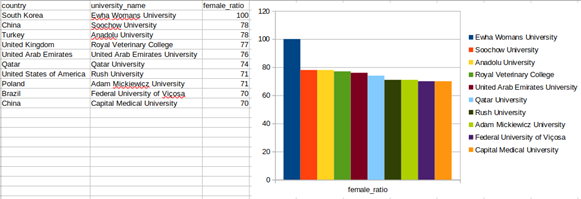
\includegraphics[width=\textwidth]{images/milepael5/resUniFemRatio.png}
\end{figure}

% Aggregering 2 %
\textbf{Andre Aggregering}\\
Denne er tilsvarende forrige aggregering, men denne gangen for mannlige studenter.

\code{Scala}{code/milepael5/universityByMaleRatio.scala}
\FigureCounter
\begin{figure}[H]
    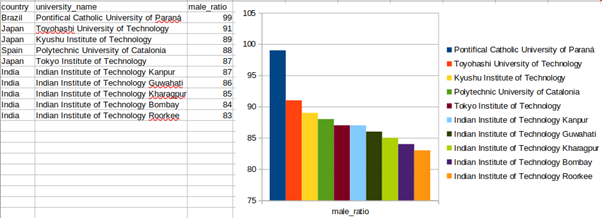
\includegraphics[width=\textwidth]{images/milepael5/resUniMaleRatio.png}
\end{figure}

% Aggregering 3 %
\textbf{Tredje Aggregering}\\
Til slutt har vi laget aggregeringen fra milepæl 4 "Average Score Per Year". Dessverre har jeg glemt å lagre scala-koden, men her er uansett resultatet i LibreOffice:

\FigureCounter
\begin{figure}[H]
    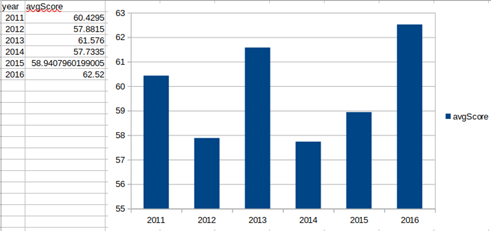
\includegraphics[scale=1]{images/milepael5/avgScoreTotStudentsActual.png}
\end{figure}


\subsubsection{Government Types Of The World (Grafdatabase)}
Begynner med å lese csv filene. Merk at i dette datasettet er det 4 forskjellige csv-filer. Så skrive de til parquet filer.

\code{Scala}{code/milepael5/readWriteREIGN.scala}

% Aggregering 1 %
\textbf{Første Aggregering}\\
Her lagde jeg kun en aggregering "Regyme Type Development" fra milepæl 4. Aggregeringen viser hvordan hver styremåte har utviklet seg i popularitet gjennom årene.

\code{Scala}{code/milepael5/governmentPopularityFirst.scala}

Til å begynne med grupperes den først på år, så på styremåte, og så telles antall opplistinger. Men dessverre var ikke dette optimalt for lesing av grafiske programmer (excel, libreoffice). Vi lagde en ny versjon hvor den har en kolonne for år og kolonner for hver styremåte. Da ble aggregeringen slik:

\code{Scala}{code/milepael5/governmentPopularityByYear.scala}

Framstilling i libreoffice:

\FigureCounter
\begin{figure}[H]
    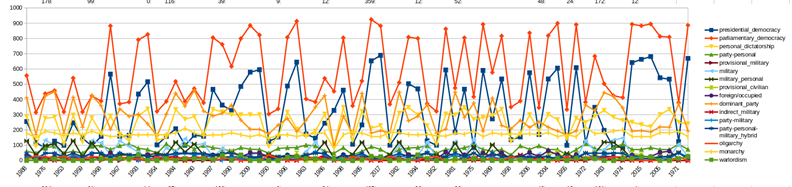
\includegraphics[width=\textwidth]{images/milepael5/libreOfficeGovPop.png}
\end{figure}

\subsubsection{Endringer på nettsiden}
Vi fant ut i denne milepælen at dynamisk brukerinput ville være vanskelig å inkorporere i noen av aggregeringene, som f.eks land-aggregeringene i dokumentdatabasene. Derfor ville det vært vesentlig mindre brukerinteraksjon på nettsiden.